% Options for packages loaded elsewhere
\PassOptionsToPackage{unicode}{hyperref}
\PassOptionsToPackage{hyphens}{url}
%
\documentclass[
]{book}
\usepackage{lmodern}
\usepackage{amssymb,amsmath}
\usepackage{ifxetex,ifluatex}
\ifnum 0\ifxetex 1\fi\ifluatex 1\fi=0 % if pdftex
  \usepackage[T1]{fontenc}
  \usepackage[utf8]{inputenc}
  \usepackage{textcomp} % provide euro and other symbols
\else % if luatex or xetex
  \usepackage{unicode-math}
  \defaultfontfeatures{Scale=MatchLowercase}
  \defaultfontfeatures[\rmfamily]{Ligatures=TeX,Scale=1}
\fi
% Use upquote if available, for straight quotes in verbatim environments
\IfFileExists{upquote.sty}{\usepackage{upquote}}{}
\IfFileExists{microtype.sty}{% use microtype if available
  \usepackage[]{microtype}
  \UseMicrotypeSet[protrusion]{basicmath} % disable protrusion for tt fonts
}{}
\makeatletter
\@ifundefined{KOMAClassName}{% if non-KOMA class
  \IfFileExists{parskip.sty}{%
    \usepackage{parskip}
  }{% else
    \setlength{\parindent}{0pt}
    \setlength{\parskip}{6pt plus 2pt minus 1pt}}
}{% if KOMA class
  \KOMAoptions{parskip=half}}
\makeatother
\usepackage{xcolor}
\IfFileExists{xurl.sty}{\usepackage{xurl}}{} % add URL line breaks if available
\IfFileExists{bookmark.sty}{\usepackage{bookmark}}{\usepackage{hyperref}}
\hypersetup{
  pdftitle={Statistics with R},
  pdfauthor={Krisna Gupta; Donny Pasaribu},
  hidelinks,
  pdfcreator={LaTeX via pandoc}}
\urlstyle{same} % disable monospaced font for URLs
\usepackage{color}
\usepackage{fancyvrb}
\newcommand{\VerbBar}{|}
\newcommand{\VERB}{\Verb[commandchars=\\\{\}]}
\DefineVerbatimEnvironment{Highlighting}{Verbatim}{commandchars=\\\{\}}
% Add ',fontsize=\small' for more characters per line
\usepackage{framed}
\definecolor{shadecolor}{RGB}{248,248,248}
\newenvironment{Shaded}{\begin{snugshade}}{\end{snugshade}}
\newcommand{\AlertTok}[1]{\textcolor[rgb]{0.94,0.16,0.16}{#1}}
\newcommand{\AnnotationTok}[1]{\textcolor[rgb]{0.56,0.35,0.01}{\textbf{\textit{#1}}}}
\newcommand{\AttributeTok}[1]{\textcolor[rgb]{0.77,0.63,0.00}{#1}}
\newcommand{\BaseNTok}[1]{\textcolor[rgb]{0.00,0.00,0.81}{#1}}
\newcommand{\BuiltInTok}[1]{#1}
\newcommand{\CharTok}[1]{\textcolor[rgb]{0.31,0.60,0.02}{#1}}
\newcommand{\CommentTok}[1]{\textcolor[rgb]{0.56,0.35,0.01}{\textit{#1}}}
\newcommand{\CommentVarTok}[1]{\textcolor[rgb]{0.56,0.35,0.01}{\textbf{\textit{#1}}}}
\newcommand{\ConstantTok}[1]{\textcolor[rgb]{0.00,0.00,0.00}{#1}}
\newcommand{\ControlFlowTok}[1]{\textcolor[rgb]{0.13,0.29,0.53}{\textbf{#1}}}
\newcommand{\DataTypeTok}[1]{\textcolor[rgb]{0.13,0.29,0.53}{#1}}
\newcommand{\DecValTok}[1]{\textcolor[rgb]{0.00,0.00,0.81}{#1}}
\newcommand{\DocumentationTok}[1]{\textcolor[rgb]{0.56,0.35,0.01}{\textbf{\textit{#1}}}}
\newcommand{\ErrorTok}[1]{\textcolor[rgb]{0.64,0.00,0.00}{\textbf{#1}}}
\newcommand{\ExtensionTok}[1]{#1}
\newcommand{\FloatTok}[1]{\textcolor[rgb]{0.00,0.00,0.81}{#1}}
\newcommand{\FunctionTok}[1]{\textcolor[rgb]{0.00,0.00,0.00}{#1}}
\newcommand{\ImportTok}[1]{#1}
\newcommand{\InformationTok}[1]{\textcolor[rgb]{0.56,0.35,0.01}{\textbf{\textit{#1}}}}
\newcommand{\KeywordTok}[1]{\textcolor[rgb]{0.13,0.29,0.53}{\textbf{#1}}}
\newcommand{\NormalTok}[1]{#1}
\newcommand{\OperatorTok}[1]{\textcolor[rgb]{0.81,0.36,0.00}{\textbf{#1}}}
\newcommand{\OtherTok}[1]{\textcolor[rgb]{0.56,0.35,0.01}{#1}}
\newcommand{\PreprocessorTok}[1]{\textcolor[rgb]{0.56,0.35,0.01}{\textit{#1}}}
\newcommand{\RegionMarkerTok}[1]{#1}
\newcommand{\SpecialCharTok}[1]{\textcolor[rgb]{0.00,0.00,0.00}{#1}}
\newcommand{\SpecialStringTok}[1]{\textcolor[rgb]{0.31,0.60,0.02}{#1}}
\newcommand{\StringTok}[1]{\textcolor[rgb]{0.31,0.60,0.02}{#1}}
\newcommand{\VariableTok}[1]{\textcolor[rgb]{0.00,0.00,0.00}{#1}}
\newcommand{\VerbatimStringTok}[1]{\textcolor[rgb]{0.31,0.60,0.02}{#1}}
\newcommand{\WarningTok}[1]{\textcolor[rgb]{0.56,0.35,0.01}{\textbf{\textit{#1}}}}
\usepackage{longtable,booktabs}
% Correct order of tables after \paragraph or \subparagraph
\usepackage{etoolbox}
\makeatletter
\patchcmd\longtable{\par}{\if@noskipsec\mbox{}\fi\par}{}{}
\makeatother
% Allow footnotes in longtable head/foot
\IfFileExists{footnotehyper.sty}{\usepackage{footnotehyper}}{\usepackage{footnote}}
\makesavenoteenv{longtable}
\usepackage{graphicx,grffile}
\makeatletter
\def\maxwidth{\ifdim\Gin@nat@width>\linewidth\linewidth\else\Gin@nat@width\fi}
\def\maxheight{\ifdim\Gin@nat@height>\textheight\textheight\else\Gin@nat@height\fi}
\makeatother
% Scale images if necessary, so that they will not overflow the page
% margins by default, and it is still possible to overwrite the defaults
% using explicit options in \includegraphics[width, height, ...]{}
\setkeys{Gin}{width=\maxwidth,height=\maxheight,keepaspectratio}
% Set default figure placement to htbp
\makeatletter
\def\fps@figure{htbp}
\makeatother
\setlength{\emergencystretch}{3em} % prevent overfull lines
\providecommand{\tightlist}{%
  \setlength{\itemsep}{0pt}\setlength{\parskip}{0pt}}
\setcounter{secnumdepth}{5}
\usepackage{booktabs}
\usepackage{amsthm}
\makeatletter
\def\thm@space@setup{%
  \thm@preskip=8pt plus 2pt minus 4pt
  \thm@postskip=\thm@preskip
}
\makeatother
\usepackage[]{natbib}
\bibliographystyle{apalike}

\title{Statistics with R}
\author{Krisna Gupta\footnote{\href{mailto:krisna.gupta@anu.edu.au}{\nolinkurl{krisna.gupta@anu.edu.au}}} \and Donny Pasaribu}
\date{2020-08-10}

\begin{document}
\maketitle

{
\setcounter{tocdepth}{1}
\tableofcontents
}
\hypertarget{some-introduction}{%
\chapter{Some Introduction}\label{some-introduction}}

\hypertarget{about-this-book}{%
\section{About this book}\label{about-this-book}}

\hypertarget{what-is-this-book-and-why}{%
\subsection{What is this book and why}\label{what-is-this-book-and-why}}

Learning a statistical software can be a daunting experience for everyone. However, as the importance of data analysis is increasing, we think more talent in this sector will only benefit everyone.

This book is created using the Bookdown \citep{R-bookdown} package and is written in Rmarkdown \citep{R-rmarkdown} language. All content in this book is free to be used and distributed by anyone for learning purpose. Please credit us if you find this book to be useful.

This book handles a mainstream curriculum of undergrad statistics, therefore it is best to use this book while also doing an undergrad statistics course. We use social sciences data set to illustrate some commands in R, but it can be easily changed to data set relevant to yourself.

\hypertarget{pre-requisite}{%
\subsection{Pre-requisite}\label{pre-requisite}}

This book is intended to anyone who are interested in learning statistics using R language. It is assumed that people has zero experience with using any programing language at all. Experience with spreadsheet program such as Microsoft Excel or Google Sheet is certainly helpful but not needed.

This book will not cover a lot of the theoretical part of statistics. Readers are assumed to understand that already. A little bit of intro will be given but that is pretty much it. Readers are expected to understand already the theory behind these techniques, or are expected to learn it from elsewhere.

\hypertarget{learning-outcome}{%
\subsection{Learning outcome}\label{learning-outcome}}

Information in this book would help you to:

\begin{itemize}
\tightlist
\item
  install and update R and Rstudio with ease
\item
  input, edit, and manage dataset
\item
  visualise dataset as needed
\item
  conducting hypothesis testing
\item
  running a regression
\item
  write a report using the results from above
\end{itemize}

\hypertarget{about-r}{%
\section{About R}\label{about-r}}

\hypertarget{what-is-r}{%
\subsection{What is R}\label{what-is-r}}

R is an open source statistical package useful for doing some statistical stuff, while RStudio is a software which improve greatly our user interface when using R compared to using R GUI. RStudio also can be used to do other stuff but let's discuss that for later.

R can be used to manipulate a huge amount of data, as well as running a handful of statistical analysis such as regression which is essentially just a matrix algebra in the background. Use of command instead of point-and-click is great because it means it can be replicable with just a script (and a bit of other stuff). Great for collaboration and peer-reviewing.

\hypertarget{good-reasons-to-start-with-r}{%
\subsection{Good reasons to start with R}\label{good-reasons-to-start-with-r}}

R is a bit behind in popularity compared to a more general language such as python or javascript. However, R is generally used among researchers, so there are many people in \href{https://campus.sagepub.com/blog/where-should-i-start-r-or-python}{academics setting use R}. R is a bit more specialised on statistical purpose. If you are learning statistics, it is easier to learn using r compared to more general programming language. If you want to learn other language later, it is easier to start with R.

Here's a more comprehensive reasons on why you should learn R from \href{https://cfss.uchicago.edu/setup/what-is-r/}{University of Chicago}.

\hypertarget{computer-requirements}{%
\subsection{Computer requirements}\label{computer-requirements}}

R and RStudio is really light you can install them in your microwave. R and RStudio supports Windows, Mac and Linux. Also, good internet connection never hurts.

\hypertarget{installing-r-and-rstudio}{%
\subsection{Installing R and RStudio}\label{installing-r-and-rstudio}}

You can easily google to get your R and RStudio installer. But we will give you links anyway. Get your R installation \href{https://cran.r-project.org/bin/windows/base/}{here if you are windows user}, \href{https://cran.r-project.org/bin/macosx/}{here for Mac users}, and \href{https://www.digitalocean.com/community/tutorials/how-to-install-r-on-ubuntu-18-04-quickstart}{here for ubuntu users}. Get your RStudio from \href{https://rstudio.com/products/rstudio/download/\#download}{this links}.

We are using recommended setting when we install R to our machine, and we suggest you do too.

\hypertarget{about-the-authors}{%
\section{About the authors}\label{about-the-authors}}

We are nobody.

\hypertarget{starting-with-r}{%
\chapter{Starting with R}\label{starting-with-r}}

🚧 Under Construction 🚧

Now that you have R and RStudio installed, let's start playing around with it. It is easy to be scared with command-type type of language, but do not worry. The first step is always the hardest. You will get there in no time at all.

One thing to note is that you will never have to use R GUI. Just keep RStudio's shortcut in your desktop and everything will be allright.

Now let's get to RStudio

\hypertarget{rstudios-interface}{%
\section{RStudio's interface}\label{rstudios-interface}}

First, familiarise yourself with RStudio interface. RStudio looks like this:
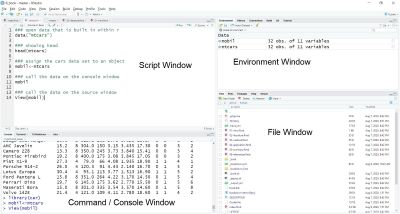
\includegraphics{tampilanR2.JPG}
As you can see from the above figure, RStudio have four main windows.

\hypertarget{console-window}{%
\subsection{console window}\label{console-window}}

Arguably the most important window in RStudio. We write R command in this window.

\hypertarget{script-window}{%
\subsection{script window}\label{script-window}}

Forget what we said about the previous window. This is the most important window in RStudio. We write our sets of command in this window

\hypertarget{environment-window}{%
\subsection{environment window}\label{environment-window}}

You can observe your environment here, such as the data and variables / series you created. This window also have other useful tab such as ``history'' which can show you the history of what happens in your environment, but we will skip them for now.

\hypertarget{files-window}{%
\subsection{files window}\label{files-window}}

Although we call it `files window', this window consists of 5 tabs. The tab file shows your working directory. When you run a code that generates file such as graphics, it will be stored in this window. Plots tab shows you your latest plot.

Packages tab show you all the package that you have. You can also add new package from this tab instead of using the \texttt{install.packages()} command. In this tab, you can also activate package that you have instead of using \texttt{library()} command.

``help'' tab will show you some information about things that you ask help for when you use \texttt{?\textquotesingle{}command\textquotesingle{}} command. Will show you how it works in a minute.

Lastly, ``viewer'' tab. I actually forgot why it exists so whatever.

\hypertarget{using-your-console-window}{%
\section{using your console window}\label{using-your-console-window}}

Generally, you type commands and operators such as \texttt{print()} and \texttt{1+1} and the likes on the console window. Let's try it a bit.

If you type 1+1 in the console and hit enter, you will get:

\begin{Shaded}
\begin{Highlighting}[]
\DecValTok{1}\OperatorTok{+}\DecValTok{1}
\end{Highlighting}
\end{Shaded}

\begin{verbatim}
## [1] 2
\end{verbatim}

you can print your name in r

\begin{Shaded}
\begin{Highlighting}[]
\KeywordTok{print}\NormalTok{(}\StringTok{'Hello world! My name is Jane Doe'}\NormalTok{)}
\end{Highlighting}
\end{Shaded}

\begin{verbatim}
## [1] "Hello world! My name is Jane Doe"
\end{verbatim}

In short, chunks of code we use in this book is meant to be typed on your console window.

\hypertarget{using-r-script}{%
\section{using R script}\label{using-r-script}}

However, to be a good coder, you will, most likely, store your chunks of code on the R script.

\hypertarget{package}{%
\section{package}\label{package}}

\hypertarget{update}{%
\section{Update}\label{update}}

You need to keep your R, RStudio and your installed packages updated as much as you can. Here's how to do it using the console window.

Firstly, install a package called \texttt{installr} by typing \texttt{install.packages(\textquotesingle{}installr\textquotesingle{})} in your console window. Don't forget to hit enter. You only need to do this once. Next, call it using \texttt{library(installr)}. Calling the package will be needed to be done everytime you start a new R session (i.e., everytime you open R).

After you called it with \texttt{library()}, type \texttt{updateR()} on your console, and let it do its magic.

To keep your packages updated, you only need to click ``tools'' on the toolbar up there, then ``Check for Packages Updates\ldots{}''. Depending on how much packages you have installed on your machine, can take a while.

Keep in mind that you need to stay connected to the internet when you update your R, RStudio and packages.

\hypertarget{beginner-stuff}{%
\chapter{Beginner stuff}\label{beginner-stuff}}

🚧 Under Construction 🚧

This chapter contains instruction the most basic and useful commands in R. We also covers data types and why it matters.

\hypertarget{setting-your-preamble}{%
\section{Setting your preamble}\label{setting-your-preamble}}

Firstly, it is a good idea to start your script with a clearing environment sets of code.

\begin{Shaded}
\begin{Highlighting}[]
\CommentTok{# Close all graphics, clear memory and screen}
\KeywordTok{graphics.off}\NormalTok{(); }\KeywordTok{remove}\NormalTok{(}\DataTypeTok{list=}\KeywordTok{ls}\NormalTok{());}\KeywordTok{cat}\NormalTok{(}\StringTok{"\textbackslash{}14"}\NormalTok{);}
\end{Highlighting}
\end{Shaded}

There are three different command in this script. \texttt{graphics.off()} clears out the environment from any graphs from previous R session. the command \texttt{remove(list=ls())} is used to remove your environment from any data and variables/series that you may have. Lastly, \texttt{cat("\textbackslash{}14")} clears your console window.

You need to set your working directory

\begin{Shaded}
\begin{Highlighting}[]
\KeywordTok{setwd}\NormalTok{(}\StringTok{'your directory'}\NormalTok{)}
\end{Highlighting}
\end{Shaded}

\hypertarget{data-management}{%
\chapter{Data Management}\label{data-management}}

🚧 Under Construction 🚧

\hypertarget{inferences}{%
\chapter{Inferences}\label{inferences}}

🚧 Under Construction 🚧

\texttt{mean(price)}

\texttt{summary(price)}

\texttt{var(price)}

\texttt{sd(price)}

\texttt{cov(price,\ bedrooms)}

\texttt{cor(price,\ bedrooms)}

\hypertarget{visualisation}{%
\chapter{Visualisation}\label{visualisation}}

🚧 Under Construction 🚧

\hypertarget{plot-command}{%
\section{Plot command}\label{plot-command}}

\hypertarget{quick-plot}{%
\subsection{quick plot}\label{quick-plot}}

\hypertarget{histogram}{%
\section{histogram}\label{histogram}}

\hypertarget{quick-histogram}{%
\subsection{quick histogram}\label{quick-histogram}}

\hypertarget{pie-chart}{%
\section{pie chart}\label{pie-chart}}

\hypertarget{quick-pie-chart}{%
\subsection{quick pie chart}\label{quick-pie-chart}}

\hypertarget{box-plot}{%
\section{box plot}\label{box-plot}}

\hypertarget{quick-box-plot}{%
\subsection{quick box plot}\label{quick-box-plot}}

\hypertarget{using-ggplot2}{%
\section{using ggplot2}\label{using-ggplot2}}

\hypertarget{hypothesis-testing}{%
\chapter{Hypothesis Testing}\label{hypothesis-testing}}

🚧 Under Construction 🚧

\hypertarget{anova}{%
\chapter{ANOVA}\label{anova}}

🚧 Under Construction 🚧

\hypertarget{simple-regression}{%
\chapter{Simple Regression}\label{simple-regression}}

🚧 Under Construction 🚧

We assume you are familiar with regression or Ordinary Least Square (OLS), but let's make a quick recap on what regression is all about.

\hypertarget{univariate-regression}{%
\section{Univariate regression}\label{univariate-regression}}

is a regression between one dependent variable and one independent variable. Most textbooks use a notation \(Y\) for dependent variable, and use \(X\) as the independent variable. A univariate regression assume this form:
\[
Y_i=\alpha+\beta X_i+ e_i
\]
where \(Y_i\) is your observed dependent variable and \(X_i\) is your observed independent variable.

There are many versions of the Gauss-Markov assumption, but really there are two main thing we assume for OLS to be unbiased:

\begin{itemize}
\tightlist
\item
  error term \(e_i\) have a conditional zero mean, i.e., \(E(e_i|X_i)=0\)
\item
  error term \(e_i\) is independent and identically distributed
\end{itemize}

We call \(\alpha\) as intercept. We generally don't interpret \(\alpha\) although it is very important to include \(\alpha\) to avoid bias. We are interested in \(\beta\), as it shows the general strength of relationship between our \(X\) and our \(Y\) is. That is, we often say:

\begin{quote}
an increase of \(X\) by 1 unit, is associated with an increase of \(Y\) by \(\beta\) unit, assuming everything else constant.
\end{quote}

Mathly, \(\beta=\frac{dy}{dx}\)

\hypertarget{running-your-univariate-regression}{%
\subsection{running your univariate regression}\label{running-your-univariate-regression}}

suppose you have

\hypertarget{plotting-your-regression}{%
\subsection{plotting your regression}\label{plotting-your-regression}}

In the previous chapter, we have learned how to plot our data using \texttt{plot()}. You can add to your script a line showing your regression result

\hypertarget{multivariate-regression}{%
\section{Multivariate regression}\label{multivariate-regression}}

Multivariate regression is just like your univariate regression, but we have more independent variable than just one. Dependent variable still only one. That is:

\[
Y_i=\alpha+\beta X_i+\gamma Z_i+ e_i
\]
The interpretation is similar.

\hypertarget{running-multivariate-regression}{%
\subsection{running multivariate regression}\label{running-multivariate-regression}}

Now, instead of

unfortunately, you can't plot multivariate regression as this regression has more than two dimension.

  \bibliography{book.bib,packages.bib}

\end{document}
